% Volume III chapter: The Thorin measure in terms of the log gamma function. Sources: misc/reviews/nick-loggamma/loggamma/loggamma_chapter.tex (432 lines; sections on the Gamma term, psi(x)-x, Chebyshev's windows, the rung, Yamazato's split, the theta kernel, Binet and Poisson; the setup, the Chebyshev identity, the threshold proof, the dilations section and the code section reduced to pointers); referee report misc/research/directions/opus/vol3/LOGG.md (M1 to M8); numbers misc/vol3/verify/LOGG/results.md. Date 17 Nov 2026.
% Coordinator notes: label prefix lg:; no bibliography file (Binet 1839, Stieltjes 1889, Chebyshev 1852, Diamond and Erdos 1980, Berg, Koumandos and Pedersen (now cited as BKP19, key in ch/nc_v3_bn_bib.tex) are named in the text; Diamond and Erdos has no entry and is not named). Figure fig/v3/lg_fig.pdf copied from the draft folder: its right panel shows psi(x)-x, the Moebius sum and E(x) up to 1e5, and the endpoint values agree with the table (psi-x = 51.56, sum 5.31, E 46.25 at 1e5), the left panel R(y) is checked at y = 1, 2 by hand; the intermediate plotted values are not in results.md. Normalisation: book chart (u = w^2, atoms gamma^2, rates gamma^2, Riemann's factor 1/2 in xi); every rate and mean taken from the draft (which used rates gamma^2/2) is halved, and K = sum over gamma > 0 of gamma^{-2} = 0.0231050 is half the draft's K.
\label{lg:ch:logg}
The function $\log\Gamma$ enters the Thorin measure of the reciprocal Xi function twice. On a rung $\alpha>1$ it appears as $\log\Gamma(\frac s2)$, the Gamma factor of $\xi$. In Chebyshev's identity it appears as $\log[x]!=\log\Gamma([x]+1)$, which carries the primes. In both readings the zeros are not in the Stirling main term, and what is left is the Stirling remainder, which is built from one function, the sawtooth $\frac12-\{y\}$. This chapter rewrites objects of Volumes I and III with that function in view. The additions are elementary: $\psi(x)-x$ as a Möbius sum of Stirling remainders (Theorem~\ref{lg:thm:psi}), the exact mass of Chebyshev's windows (Theorem~\ref{lg:thm:window}), the uncompensated Yamazato split of a rung and the limit of its integer crossings under RH (Theorem~\ref{lg:thm:cross}), a splitting of a sum of exponentials into the critical points plus one picked exponential (Lemma~\ref{lg:lem:pick}, Theorem~\ref{lg:thm:split}), and the theta kernel as a sawtooth mixture of Gamma$(2)$ densities (Theorem~\ref{lg:thm:pk}). They are from an unrefereed note of Polson (November 2026). The chapter is a change of language, and nothing in it proves RH or improves the half plane $\frac78$ of \cite{OAI26a}: RH becomes a statement of square root cancellation in Möbius sums of the sawtooth.

\section{Log gamma, read twice}\label{lg:sec:twice}
Fix $\alpha>1$ and write $r=\sqrt z$. By Theorem~\ref{ct:thm:dictionary} the Thorin density of rung $\alpha$ is $t_\alpha(z)=D^\xi(r)/(2\pi r)$ with
\[
D^\xi(r)=v_\alpha(r)-b_\alpha=\Re\frac{\xi'}{\xi}(\alpha+ir)-\frac{\xi'}{\xi}(\alpha),
\]
and RH holds if and only if $t_\alpha\ge0$ on every rung $\alpha>\frac12$ (Proposition~\ref{ct:prop:qrh}). The sine squared lemma of Volume I, equation~\eqref{eq:sin2}, turns a Lévy measure into such a density. From $\xi(s)=\frac12s(s-1)\pi^{-s/2}\Gamma(\frac s2)\zeta(s)$, $D^\xi=D^{\mathrm{el}}+D^\Gamma+D^P$ is the sum of an elementary term, a Gamma term and a prime term. With the atoms
\[
d(r;c)=\int_0^\infty2\sin^2\bigl(\tfrac{rx}2\bigr)e^{-cx}\dd x=\frac{r^2}{c(c^2+r^2)}=q_c(r)\qquad(c>0)
\]
of equation~\eqref{bp:eq:excess}, $D^{\mathrm{el}}=-d(r;\alpha)\allowbreak-d(r;\alpha-1)$ and $D^P(r)=\sum_n\Lambda(n)n^{-\alpha}\allowbreak\,2\sin^2(\frac r2\log n)\ge0$. The decomposition is in Proposition~\ref{pol:prop:primes} and Theorem~\ref{nf:thm:four}. The two readings of $\log\Gamma$ are these.
\begin{center}
\small
\begin{tabular}{lll}
\toprule
 & first reading & second reading\\
\midrule
variable & $s$ on the rung & $x\ge1$ real\\
function & $\log\Gamma(\frac s2)$ & $T(x)=\log[x]!=\log\Gamma([x]+1)$\\
role & archimedean factor & primes\\
main term & $\frac s2\log\frac s2-\frac s2$ & $x\log x-x$\\
source & Binet, 1839 & Chebyshev, 1850\\
\bottomrule
\end{tabular}
\end{center}

\subsection*{First reading: the Gamma term}
The proof of Proposition~\ref{pol:prop:primes} gives, for $\alpha>0$, $D^\Gamma(r)=\sum_{k\ge0}d(r;\alpha+2k)=\int_0^\infty2\sin^2(\frac{rx}2)\frac{e^{-\alpha x}}{1-e^{-2x}}\dd x>0$, one atom for each pole of $\Gamma(\frac s2)$. The kernel is that of Binet's formula,
\[
\log\Gamma(z)=\bigl(z-\tfrac12\bigr)\log z-z+\tfrac12\log2\pi+\int_0^\infty\Bigl(\frac1{e^t-1}-\frac1t+\frac12\Bigr)e^{-tz}\frac{\dd t}t ,
\]
and Binet's kernel is $t$ times the Laplace transform of the sawtooth:
\[
\frac1{e^t-1}-\frac1t+\frac12=t\int_0^\infty\bigl(\tfrac12-\{y\}\bigr)e^{-ty}\dd y ,
\]
because $\frac1{e^t-1}=t\int_0^\infty[y]e^{-ty}\dd y$ (integrate $\int e^{-ty}\dd[y]$ by parts) and $\frac1t=t\int_0^\infty y\,e^{-ty}\dd y$. So the archimedean part of the Thorin measure is the integers minus their mean density, seen through a Laplace transform. The same device gives the Gamma term as Stirling's main term plus a positive mixture of atoms.
\begin{proposition}[the Gamma term as a mixture]\label{lg:prop:rung}
For $\alpha>0$ and $r>0$,
\[
D^\Gamma(r)=\tfrac14\log\Bigl(1+\frac{r^2}{\alpha^2}\Bigr)+\sum_{k\ge0}\int_k^{k+1}\bigl[d(r;\alpha+2k)-d(r;\alpha+2v)\bigr]\dd v,
\]
and every integrand is positive. For $\alpha>1$, $D^\xi(r)=\sum_{k\ge1}d(r;\alpha+2k)+\sum_n\Lambda(n)n^{-\alpha}\,2\sin^2(\frac r2\log n)-d(r;\alpha-1)$: the rung is a positive mixture of Gamma atoms and prime atoms minus the single atom of the pole.
\end{proposition}
\begin{proof}
The function $v\mapsto d(r;\alpha+2v)$ decreases, so each cell $[k,k+1]$ gives a positive term, and $\int_0^\infty d(r;\alpha+2v)\dd v=\frac14\log(1+r^2/\alpha^2)$. In the second display the atom $k=0$ of $D^\Gamma$ cancels $-d(r;\alpha)$ of $D^{\mathrm{el}}$.
\end{proof}
The threshold at which the Gamma atoms alone dominate the pole atom is not new here. By Proposition~\ref{pol:prop:primes}, $\sum_{k\ge1}d(r;\alpha+2k)\ge d(r;\alpha-1)$ for all $r$ if and only if $\alpha\ge\alpha_1=7.78918\ldots$, the root of $(\alpha-1)^3\zeta(3,1+\frac\alpha2)=8$; the proof compares the ratios at $r\to0$ and uses that the sum increases in $\alpha$. A cruder condition, from bounding the Gamma sum below by an integral, has its root at $8.7154$ (computed); it is sufficient and not an exact threshold. For $1<\alpha<\alpha_1$ the primes must make up the deficit, and they do for every $\alpha\ge1$ by Proposition~\ref{bp:prop:valpha}, which is proved in ball arithmetic. For $\alpha\le1$ the prime mixture diverges. It combines with the pole atom into the $2\sin^2$ transform of $\dd[\psi(e^x)-e^x]$, Chebyshev's error, which by Theorem~\ref{lg:thm:psi} below is $\dd[\sum_k\mu(k)R(e^x/k)+E(e^x)]$, a signed measure. By Proposition~\ref{ct:prop:qrh} positivity of the rung below $1$ is a zero free half plane, and the mixture representation does not decide it. Numerical checks (computed): $D^\Gamma$ by the digamma function and by the kernel agree at $(\alpha,r)=(\frac12,5)$ and $(\frac34,14.1347)$ with values $2.5710326$ and $2.3544023$; the two sides of the Binet display at $t=0.7$ are $0.0578624351$; at $(\alpha,r)=(2,5)$, $D^\Gamma=0.75354$ and $D^\xi=0.32250+0.64864-0.96154=0.00961$, equal to the value computed directly, so the margin is thin there.

\subsection*{Second reading: Chebyshev's identity}
With $\psi(x)=\sum_{p^k\le x}\log p$, Chebyshev's identity is $T(x)=\log[x]!=\sum_{k\ge1}\psi(x/k)$, equation~\eqref{ct:eq:cheb}. Möbius inversion (Theorem~\ref{ct:thm:mobius}(1)) gives the primes from $\log\Gamma$,
\[
\psi(x)=\sum_{k\le x}\mu(k)\log\Gamma\Bigl(\Bigl[\frac xk\Bigr]+1\Bigr),\qquad-\zeta'(s)=\int_1^\infty x^{-s}\dd\log\Gamma([x]+1).
\]
Computed: $T(10^5)=1051299.2219$ equals $\sum_k\psi(10^5/k)$, and the inverted sum reproduces $\psi(10^6)=999586.5975$ to ten digits.

\section{The term $\psi(x)-x$}\label{lg:sec:psi}
Let $R$ be the Stirling remainder of $\log[y]!$,
\[
R(y)=\log\Gamma([y]+1)-(y\log y-y),\qquad y>0,
\]
and put $m(x)=\sum_{k\le x}\mu(k)/k$, $\ell(x)=\sum_{k\le x}\mu(k)\log k/k$. The theorem rewrites the Möbius inversion of Chebyshev's identity with the main terms moved out.
\begin{theorem}[proved: Möbius sum of Stirling remainders]\label{lg:thm:psi}
For every $x\ge1$,
\[
\psi(x)-x=\sum_{k=1}^\infty\mu(k)\,R\Bigl(\frac xk\Bigr),
\]
a conditionally convergent series, where for $y<1$ the remainder is $R(y)=y-y\log y$. The part $k\le x$ involves $\log\Gamma$ at integers, and the tail is explicit:
\[
E(x):=\sum_{k>x}\mu(k)\,R\Bigl(\frac xk\Bigr)=x\bigl[(\log x-1)\,m(x)-\ell(x)-1\bigr].
\]
The tail satisfies $E(x)=o(x)$, since $m(x)\log x\to0$ and $\ell(x)\to-1$ (the prime number theorem with the de la Vallée Poussin error term, as in the proof of Theorem~\ref{ct:thm:mobrate}). For $y\ge1$,
\[
R(y)=1+\bigl(\tfrac12-\{y\}\bigr)\log y+\int_1^y\bigl(\{t\}-\tfrac12\bigr)\frac{\dd t}t=\bigl(\tfrac12-\{y\}\bigr)\log y+\tfrac12\log2\pi+O(1/y).
\]
\end{theorem}
\begin{proof}
Insert $T(y)=R(y)+y\log y-y$ in $\psi(x)=\sum_{k\le x}\mu(k)T(x/k)$; the main terms give $x(\log x-1)m(x)-x\ell(x)$, so $\psi(x)-x=\sum_{k\le x}\mu(k)R(x/k)+x[(\log x-1)m(x)-\ell(x)-1]$. For the tail, $R(x/k)=-\frac xk(\log x-\log k-1)$ when $k>x$, and $\sum_{k>x}\mu(k)/k=-m(x)$, $\sum_{k>x}\mu(k)\log k/k=-1-\ell(x)$, by $\sum\mu(k)/k=0$ and $\sum\mu(k)\log k/k=-1$; this gives the same bracket. For the sawtooth form, $T(y)=\int_{1^-}^y\log t\dd[t]=\int_1^y\log t\dd t+\int_1^y\log t\dd([t]-t)$, and an integration by parts gives $-\{y\}\log y+\int_1^y\{t\}\frac{\dd t}t$; the constant is $\int_1^\infty(\{t\}-\frac12)\frac{\dd t}t=\frac12\log2\pi-1$.
\end{proof}
The following table is computed (floating point over a sieve to $10^7$, two precisions), and its rows add up.
\begin{center}
\small
\begin{tabular}{rrrrr}
\toprule
$x$ & $\psi(x)-x$ & $\sum_{k\le x}\mu(k)R(x/k)$ & $E(x)$ & sum\\
\midrule
$10^2$ & $-5.955$ & $-2.945$ & $-3.010$ & $-5.955$\\
$10^3$ & $-3.319$ & $0.686$ & $-4.005$ & $-3.319$\\
$10^4$ & $13.397$ & $-7.707$ & $21.104$ & $13.397$\\
$10^5$ & $51.564$ & $5.315$ & $46.249$ & $51.564$\\
$10^6$ & $-413.403$ & $-198.949$ & $-214.453$ & $-413.403$\\
\bottomrule
\end{tabular}
\end{center}
The sum over $k\le x$ has $x$ terms of size about $\log$; with absolute values it is of order $x$, and with the signs of $\mu$ it is of order $\sqrt x$ in this range. The tail $E(x)$ is of the same size as the sum over $k\le x$: it is the tail of the same series, and the series converges only at the rate of the prime number theorem. For $x=100$ the partial sums to $N=10^2,10^3,10^5,10^6,10^7$ are $-2.94$, $-4.54$, $-6.34$, $-5.75$, $-5.83$, against $\psi(x)-x=-5.95$ (computed).
\begin{figure}[t]
\centering
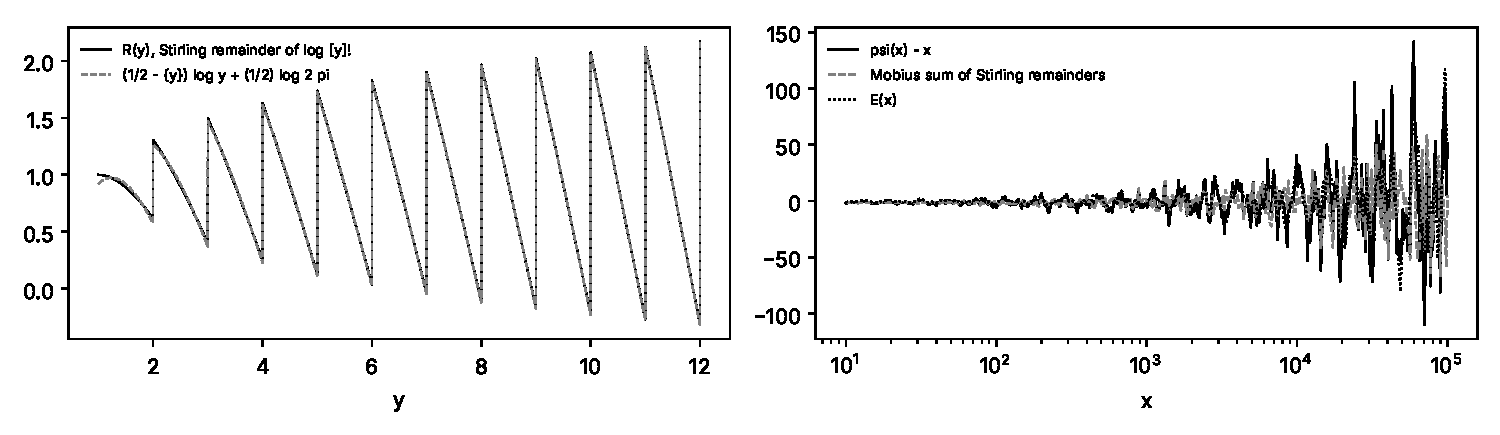
\includegraphics[width=\textwidth]{fig/v3/lg_fig.pdf}
\caption{Left: the Stirling remainder $R(y)$ of $\log[y]!$ and its sawtooth form. Right: $\psi(x)-x$, the Möbius sum of Stirling remainders, and $E(x)$, for $10\le x\le10^5$.}
\label{lg:fig:remainder}
\end{figure}

\subsection*{Where $\psi(x)-x$ lives}
Write $y=x/k$ and $f=\{y\}$, and expand the Stirling remainder as $R(y)=(\frac12-f)\log y+\frac12\log2\pi+J([y])+\cdots$, with Binet's function $J$ defined by $\log n!=(n+\frac12)\log n-n+\frac12\log2\pi+J(n)$. The error then splits into five Möbius sums (computed):
\begin{center}
\small
\begin{tabular}{lrrr}
\toprule
piece & $x=10^5$ & $x=10^6$ & $x=10^7$\\
\midrule
$\psi(x)-x$ & $51.6$ & $-413.4$ & $-1460.6$\\
main, $\sum\mu(k)(y\log y-y)-x$, which is $E(x)$ & $46.2$ & $-214.5$ & $-1042.1$\\
sawtooth, $\sum\mu(k)(\frac12-f)\log y$ & $54.4$ & $-404.2$ & $-1442.3$\\
constant, $\frac12\log2\pi\cdot M(x)$ & $-44.1$ & $194.8$ & $952.9$\\
Binet, $\sum\mu(k)J([x/k])$ & $-4.8$ & $19.2$ & $115.1$\\
remainder & $-0.2$ & $-8.9$ & $-44.3$\\
\bottomrule
\end{tabular}
\end{center}
Here $M(x)=\sum_{k\le x}\mu(k)$ is the Mertens function, $M(10^7)=1037$. Every row is a Möbius weighted sum of the same order as the error, and the rows nearly cancel. So a finer Stirling expansion does not give a finer error: each Stirling term, summed against $\mu$, becomes a weighted Mertens sum. Under RH these are $O(x^{1/2+\varepsilon})$; that they are no smaller is a heuristic, not a result. The Binet row is not small because it comes from large $k$, where $[x/k]=1,2,3,\dots$ and $J$ is not small; it equals $\sum_jJ(j)[M(x/j)-M(x/(j+1))]$. The $\sqrt x$ fluctuation is arithmetic, set by the zeros and equivalently by $M$, and not by the analytic expansion of $\log\Gamma$. So one sawtooth drives both parts of the Thorin measure. For the Gamma term it is smoothed by a Laplace transform and positivity is free. For the primes it is multiplied by $\log y$ and sieved by $\mu$, and the whole difficulty is there. Precision in $\log\Gamma$ pays where the weights are finite, as in the next section.

\section{Chebyshev's windows}\label{lg:sec:windows}
A sum minus its integral is a mixture over the unit cells, $\sum_{n\ge1}f(n)-\int_0^\infty f(v)\dd v=\sum_{n\ge1}\int_{n-1}^n(f(n)-f(v))\dd v$, and if $f$ is monotone every cell has the same sign. This is the device of Lemma~\ref{ct:lem:split} and of Proposition~\ref{lg:prop:rung}. Here it is used for Chebyshev's combination of floors. Let $c=(1,-1,-1,-1,1)$ on $k=1,2,3,5,30$, so that $\sum c_k/k=0$ and $A=-\sum c_k\log k/k=0.92129$ (Proposition~\ref{ct:prop:cheb1850}), and
\[
U(y)=[y]-\bigl[\tfrac y2\bigr]-\bigl[\tfrac y3\bigr]-\bigl[\tfrac y5\bigr]+\bigl[\tfrac y{30}\bigr].
\]
By Proposition~\ref{ct:prop:cheb1850}, $U$ takes only the values $0$ and $1$. It equals $1$ on the intervals $[a_j,b_j)=[1,6),[7,10),[11,12),[13,15),[17,18),[19,20),[23,24),[29,30)$, and then with period $30$. By Theorem~\ref{ct:thm:chebME}, $e^{-Aw}\Gamma(1+w)\Gamma(1+\frac w{30})/[\Gamma(1+\frac w2)\Gamma(1+\frac w3)\Gamma(1+\frac w5)]=\prod_j\frac{1+w/b_j}{1+w/a_j}=\sum_jp_j\frac{a_j}{a_j+w}$, a mixture of exponentials of mean $A$, with Lévy density $K(s)/s$,
\[
K(s)=\sum_kc_k\frac1{e^{ks}-1}=\sum_j\bigl(e^{-a_js}-e^{-b_js}\bigr),\qquad e^{-s}-e^{-6s}\le K(s)\le e^{-s}
\]
(the bounds hold on a grid $0.001\le s\le8$, computed). The first six weights are $p_j=0.9175$, $0.0141$, $0.0034$, $0.0041$, $0.0028$, $0.0016$ at the rates $a_j=1,7,11,13,17,19$; they are the first six of infinitely many, with the rates $23,29,31,\dots$ following, and they sum to $0.9435$ (computed).
\begin{theorem}[proved: the Chebyshev error on the windows]\label{lg:thm:window}
Let $W(x)=\bigcup_j(\frac x{b_j},\frac x{a_j}]$. Then $W(x)$ has length exactly $Ax$ and
\[
\int_{W(x)}\dd\bigl(\psi(t)-t\bigr)=\sum_{k\in\{1,2,3,5,30\}}c_k\,R\Bigl(\frac xk\Bigr),
\]
with no error term. In smooth form, as $t\to0$,
\[
\int_0^\infty K(yt)\,\dd\bigl(\psi(y)-y\bigr)=\sum_m\Lambda(m)K(mt)-\frac At\longrightarrow-\tfrac12\log2\pi .
\]
\end{theorem}
\begin{proof}
Since $T(y)=\sum_m\Lambda(m)[y/m]$, $\sum_kc_kT(x/k)=\sum_m\Lambda(m)U(x/m)$, and $U(x/m)=1$ exactly when $m\in W(x)$: the left side is the $\psi$ mass of the windows. The length of $W(x)$ is $x\int_1^\infty U(y)y^{-2}\dd y=Ax$, the constants cancelling by $\sum c_k/k=0$. And $\sum_kc_k[(x/k)\log(x/k)-x/k]=Ax$ for the same reason, so $\sum_kc_kT(x/k)-Ax=\sum_kc_kR(x/k)$. For the smooth form, $\sum_m\Lambda(m)K(mt)=\sum_kc_kL(kt)$ with $L(t)=\sum_n\log n\,e^{-nt}=-(\log t+\gamma)/t+\frac12\log2\pi+O(t)$, from the poles of $\Gamma(s)(-\zeta'(s))$ at $s=1$ and $s=0$, and $\sum c_k=-1$.
\end{proof}
The window error is computed as follows, next to the full error (both computed, the first column agrees with the direct mass minus $Ax$ to the printed digits).
\begin{center}
\small
\begin{tabular}{rrr}
\toprule
$x$ & error on the windows & full error $\psi(x)-x$\\
\midrule
$10^3$ & $-3.607$ & $-3.319$\\
$10^4$ & $-4.757$ & $13.397$\\
$10^5$ & $-5.908$ & $51.564$\\
$10^6$ & $-7.059$ & $-413.403$\\
\bottomrule
\end{tabular}
\end{center}
The windows have density $0.921$ in $(0,x]$, and the error integrated over them is close to $-\frac12\log x$ (computed values above, against $-3.45$ to $-6.91$). The whole of the $\sqrt x$ fluctuation lives on the complementary windows, of density $7.9\%$: with $e(x)=\psi(x)-x$, $e(x)=\sum_kc_kR(x/k)+\sum_j[e(x/b_j)-e(x/a_{j+1})]$. The smoothed error is $-1.1343$, $-0.9523$, $-0.9224$, $-0.9196$ at $t=0.1,0.01,0.001,0.0002$ (computed), against the limit $-0.9189$: against the positive kernel $K$ the Chebyshev error is bounded, with no logarithm. Probabilistically $K(mt)$ is the probability that $m$ falls in $W(x)$ when $x$ is an exponential variable divided by $t$. With Robbins' bounds \cite{Robbins55}, $\frac1{12n+1}<J(n)<\frac1{12n}$, the window error can be bounded: at $x=10^6$ the elementary part is $-7.0591684$ (floating point) and the $J$ part lies in $[1.750018,1.750025]\times10^{-6}$ (computed).

That the windows do not see the zeros is Proposition~\ref{ct:prop:mellincheb} and the remark after it: the zeros of $\zeta$ cancel in $-\zeta'P$. What the log gamma reading adds is a convergent expansion with no zero terms.
\begin{proposition}[proved: the windows are blind to the zeros]\label{lg:prop:blind}
The kernel $K$ has Mellin transform $\Gamma(s)\zeta(s)C(s)$ with $C(s)=\sum_kc_kk^{-s}$, so that this transform vanishes at every zero of $\zeta$. Hence $\sum_m\Lambda(m)K(mt)$ has Mellin transform $-\Gamma(s)\zeta'(s)C(s)$, with no pole at any zero, and
\[
\sum_m\Lambda(m)K(mt)-\frac At=-\tfrac12\log2\pi+\sum_{n\ge1}\frac{(-1)^{n+1}\zeta'(-n)}{n!}\,C(-n)\,t^n ,
\]
a series convergent for $0<t<2\pi/30$, with $C(-n)=1-2^n-3^n-5^n+30^n$; its first term is $-3.4738\,t$.
\end{proposition}
\begin{proof}
$L(t)=\sum_k\log k\,e^{-kt}$ has Mellin transform $-\Gamma(s)\zeta'(s)$. Moving the contour to the left past the poles at $s=1$, $s=0$ and $s=-n$ gives $L(t)=-(\log t+\gamma)/t+\frac12\log2\pi+\sum_{n\ge1}(-1)^{n+1}\zeta'(-n)t^n/n!$, convergent for $|t|<2\pi$ by the functional equation. Apply it to $\sum_kc_kL(kt)$, with $\sum c_k/k=0$, $\sum c_k\log k/k=-A$ and $\sum c_k=-1$.
\end{proof}
At $t=0.05$, $0.01$, $0.001$ the series to twelve terms gives $-1.0584095034$, $-0.9523417592$, $-0.9223992149$, and the direct sums over the prime powers to $10^7$ give $-1.0584095006$, $-0.9523417592$, $-0.9223992149$ (computed). The Möbius combination of Theorem~\ref{ct:thm:mobius} has kernel $e^{-s}$ itself, and then the zeros return, each damped by $\Gamma(\rho)$: $\sum_m\Lambda(m)e^{-m/X}=X-\sum_\rho\Gamma(\rho)X^\rho-\log2\pi+1.98505/X+\cdots$. At $X=10^5$ the residual after the analytic terms is about $2.8\times10^{-7}$, and the first forty zeros account for it; $|\Gamma(\rho_1)|=5.7\times10^{-10}$ (computed). The smoothing that makes Stirling's series convergent is the same decay that buries the fluctuation.

\section{Yamazato's split of a rung}\label{lg:sec:split}
Two distribution functions are in use for the same rung, and they must not be confused. Let $v_\alpha(r)=\Re\frac{\xi'}{\xi}(\alpha+ir)$ and $b_\alpha=\frac{\xi'}{\xi}(\alpha)$. The compensated function of Section~\ref{ct:sec:yamazato}, used in Proposition~\ref{ct:prop:yamxi} and Conjecture~\ref{ct:conj:canonical}, is
\[
F_\alpha(R)=\frac1\pi\bigl(\arg\xi(\alpha+iR)-R\,b_\alpha\bigr),
\]
the distribution function in $r$ of the Thorin density $(v_\alpha-b_\alpha)/\pi$. This chapter also uses the uncompensated function
\[
F^{\mathrm u}_\alpha(R)=\frac1\pi\arg\xi(\alpha+iR)=\frac1\pi\int_0^Rv_\alpha(r)\dd r ,
\]
the argument taken continuously from $\arg\xi(\alpha)=0$. Since $\frac1\pi\int_0^\infty\log(1+w^2/r^2)\dd r=w$, a Thorin density $v_\alpha/\pi$ in $r$ has Laplace exponent $\log\frac{\xi(\alpha+\sqrt u)}{\xi(\alpha)}$ in $u=w^2$. So when $v_\alpha\ge0$ there is a variable $X^\xi_\alpha$ with
\[
\mathbb Ee^{-uX^\xi_\alpha}=\frac{\xi(\alpha)}{\xi(\alpha+\sqrt u)},
\]
a GGC; it is the variable $T_\alpha=S_\alpha+T_\alpha^\circ$ of Proposition~\ref{bp:prop:valpha}, with the stable part $S_\alpha$ included, whereas the compensated variable is $T^\circ_\alpha$. The condition $v_\alpha\ge0$ is $\Re\frac{\xi'}{\xi}(\alpha+ir)\ge0$ for all $r$, which holds for every $\alpha\ge1$ and for every $\alpha>\Theta$, term by term in the sum over zeros. By Lagarias \cite{Lagarias} it holds for every $\alpha>\frac12$ if and only if RH does. It is weaker, rung by rung, than the compensated condition $t_\alpha\ge0$ of Proposition~\ref{ct:prop:qrh}, which is also equivalent to RH only over all $\alpha>\frac12$. Taking arguments in the definition of $\xi$,
\[
F^{\mathrm u}_\alpha(R)=\frac1\pi\Im\log\Gamma\Bigl(\frac{\alpha+iR}2\Bigr)-\frac R{2\pi}\log\pi+\frac1\pi\arg\bigl(s(s-1)\bigr)+\frac1\pi\arg\zeta(\alpha+iR),
\]
so the smooth count of zeros is an imaginary part of $\log\Gamma$, and the primes contribute the fluctuation (compare Theorem~\ref{dz:thm:mass}, which names the remainder). At $(\alpha,R)=(\frac34,50)$ the first two terms together are $8.4857$ and, with principal arguments, the last two are $0.9968$ and $0.2949$; the total is $9.777$ (computed). The split of Lemma~\ref{ct:lem:split} applied to $F^{\mathrm u}_\alpha$ gives, where $v_\alpha\ge0$,
\[
X^\xi_\alpha\overset d=\sum_j\mathrm{Exp}\bigl(R_j^2\bigr)+M_\alpha,\qquad F^{\mathrm u}_\alpha(R_j)=j,
\]
with $M_\alpha$ a mixture of exponentials whose Steutel function is $\{F^{\mathrm u}_\alpha\}\in[0,1)$. The crossings are these (computed from the zeros; $F^{\mathrm u}_\alpha$ is monotone on the grid at the three levels).
\begin{center}
\small
\begin{tabular}{lrrrrr}
\toprule
crossings $R_j$, $\alpha=2$ & $15.155$ & $21.559$ & $25.827$ & $30.614$ & $33.800$\\
$\alpha=1$ & $15.538$ & $22.038$ & $26.222$ & $31.161$ & $34.147$\\
$\alpha=\frac34$ (under RH) & $15.574$ & $22.083$ & $26.260$ & $31.214$ & $34.182$\\
zeros $\kappa_j$ of $\Xi'$ & $15.586$ & $22.098$ & $26.272$ & $31.232$ & $34.193$\\
zeros $\gamma_j$ of $\Xi$ & $14.135$ & $21.022$ & $25.011$ & $30.425$ & $32.935$\\
\bottomrule
\end{tabular}
\end{center}
As $\alpha\downarrow\frac12$ the crossings of $F^{\mathrm u}_\alpha$ tend to the zeros of $\Xi'$. This is to be set beside Conjecture~\ref{ct:conj:canonical}: for the compensated $F_\alpha$ the limits are the critical points $18.544,23.688,\dots$ of the canonical product, and the critical points $15.59,22.10,\dots$ of $\Xi$ itself are the limits for the uncompensated one.
\begin{theorem}[conditional on RH: the crossings tend to the critical points]\label{lg:thm:cross}
Assume RH and that the zeros $\gamma_j$ and $\gamma_{j+1}$ are simple. Let $R_j(\alpha)$ solve $F^{\mathrm u}_\alpha(R_j)=j$. Then $R_j(\alpha)\to\kappa_j$ as $\alpha\downarrow\frac12$, where $\kappa_j$ is the zero of $\Xi'$ in $(\gamma_j,\gamma_{j+1})$.
\end{theorem}
\begin{proof}
Put $a=\alpha-\frac12$. Under RH, $\Re\,\xi'/\xi(\alpha+ir)=\sum_\gamma a/(a^2+(r-\gamma)^2)$ over all zeros, so $F^{\mathrm u}_\alpha(R)=\frac1\pi\sum_{\gamma>0}[\arctan\frac{R-\gamma}a+\arctan\frac{R+\gamma}a]$, which is increasing. For $R$ in a compact subset of $(\gamma_j,\gamma_{j+1})$, $\arctan\frac xa=\frac\pi2\,\mathrm{sgn}\,x-\frac ax+O(a^3/|x|^3)$ gives
\[
F^{\mathrm u}_\alpha(R)=j-\frac a\pi\,\frac{\Xi'}{\Xi}(R)+O(a^3),\qquad\frac{\Xi'}{\Xi}(R)=\sum_{\gamma>0}\Bigl(\frac1{R-\gamma}+\frac1{R+\gamma}\Bigr),
\]
uniformly. On $(\gamma_j,\gamma_{j+1})$ the function $\Xi'/\Xi$ decreases strictly from $+\infty$ to $-\infty$ and vanishes only at $\kappa_j$, and $F^{\mathrm u}_\alpha(\gamma_j)\to j-\frac12$, $F^{\mathrm u}_\alpha(\gamma_{j+1})\to j+\frac12$. Take a compact interval in the gap with $\kappa_j$ in its interior; for small $a$ the function $F^{\mathrm u}_\alpha-j$ is negative at its left end and positive at its right end, and it is increasing, so the unique solution of $F^{\mathrm u}_\alpha(R)=j$ lies in the interval. Shrinking the interval gives the convergence to $\kappa_j$.
\end{proof}
\begin{remark}[a possible bearing on the canonical product]\label{lg:rem:canonical}
Conjecture~\ref{ct:conj:canonical} leaves open the uniformity in $r$ of the expansion in $\epsilon=\alpha-\frac12$. The proof above supplies that uniformity for $F^{\mathrm u}_\alpha$. For the compensated $F_\alpha$ the same expansion reads $F_\alpha=j-\frac a\pi(\frac{\Xi'}\Xi(R)+qR)+O(a^2)$ on compact subsets of a gap, with $b_\alpha=qa+O(a^2)$, and under RH $F_\alpha$ is increasing because $t_\alpha\ge0$ (Proposition~\ref{ct:prop:qrh}). If the sign change of $\frac{\Xi'}\Xi+qR$ on a gap is as in the heuristic derivation, the argument of the proof would carry over. We have not checked this and make no claim: Conjecture~\ref{ct:conj:canonical} stays a conjecture here.
\end{remark}
On the line itself the split is exact, and it is a general fact about sums of exponentials.
\begin{lemma}[proved: critical points and one pick]\label{lg:lem:pick}
Let $z_1\le z_2\le\cdots$ be positive with $m=\sum1/z_j<\infty$, and $f(u)=\prod(1+u/z_j)$. Then $f'$ has only negative zeros $-z'_j$, interlacing those of $f$, and
\[
\sum_j\mathrm{Exp}(z_j)\overset d=\sum_j\mathrm{Exp}(z'_j)+\mathrm{Exp}(z_J),\qquad P(J=j)=\frac1{m\,z_j},
\]
with all variables independent.
\end{lemma}
\begin{proof}
$f$ is of genus zero with negative zeros, so $f'$ is too, by Laguerre's theorem, and $f'(u)=f'(0)\prod(1+u/z'_j)$. Write $\frac1{f(u)}=\frac{f'(0)}{f'(u)}\cdot\frac{f'(u)}{f'(0)f(u)}$. The first factor is the Laplace transform of $\sum\mathrm{Exp}(z'_j)$, and since $f'/f=\sum1/(z_j+u)$ and $f'(0)=m$, the second is $\sum_j\frac1{mz_j}\frac{z_j}{z_j+u}$.
\end{proof}
The picked law is the case $k=1$ of Remark~\ref{rem:maxexp:kolmogorov}, where the weights proportional to $\gamma^{-2k}$ appear.
\begin{theorem}[conditional on RH: the split on the critical line]\label{lg:thm:split}
Let $H=2T$ be the Brownian clock of Section~\ref{ch:clock} as elsewhere in this volume, with $\mathbb Ee^{-uH}=\xi(\frac12)/\xi(\frac12+\sqrt{2u})$, which under RH is $\sum_{\gamma>0}\mathrm{Exp}(\gamma^2/2)$ ($T$ itself is not used, since $T$ denotes $\log[x]!$). Assume RH, let $0<\kappa_1<\kappa_2<\cdots$ be the positive zeros of $\Xi'$ and $K=\sum_{\gamma>0}\gamma^{-2}=0.0231050$ (computed). Then
\[
H\overset d=\sum_j\mathrm{Exp}\bigl(\kappa_j^2/2\bigr)+\mathrm{Exp}\bigl(\gamma_J^2/2\bigr),\qquad P(J=j)=\frac{1}{K\gamma_j^2},
\]
with all variables independent. The weights are $0.2166$, $0.0979$, $0.0692$, $0.0468$, $0.0399,\dots$, and the means of the two parts are $0.04299$ and $0.00322$ (computed from the zeros).

More generally let $g(u)=\xi(\frac12+\sqrt{2u})/\xi(\frac12)=\sum_ne_nu^n$. For every $n\ge0$ the derivative $g^{(n)}$ has only negative zeros $-(\kappa^{(n)}_j)^2/2$, the variable $H^{(n)}=\sum_j\mathrm{Exp}((\kappa^{(n)}_j)^2/2)$ has mean $(n+1)e_{n+1}/e_n$, decreasing to zero, and
\[
H\overset d=\sum_{n\ge0}\mathrm{Exp}\bigl((\kappa^{(n)}_{J_n})^2/2\bigr),
\]
a convergent sum of independent variables, one for each derivative of $g$, where $J_n$ picks a zero of $g^{(n)}$ with probability proportional to $(\kappa^{(n)}_j)^{-2}$.
\end{theorem}
\begin{proof}
Under RH, $g(u)=\prod_{\gamma>0}(1+2u/\gamma^2)$, and $\Xi'(t)/t=-\Xi(0)g'(u)$ at $u=-t^2/2$, so the zeros of $g'$ are at $-\kappa_j^2/2$. The first statement is Lemma~\ref{lg:lem:pick} with $z_j=\gamma_j^2/2$ and $m=2K$, whose weights $1/(mz_j)=1/(K\gamma_j^2)$ are the stated ones. Applying the lemma to $g^{(n)}$ for $n=0,1,\dots,N-1$ gives $H=\sum_{n<N}\mathrm{Exp}((\kappa^{(n)}_{J_n})^2/2)+H^{(N)}$ with independent terms. The mean of $H^{(n)}$ is $g^{(n+1)}(0)/g^{(n)}(0)=(n+1)e_{n+1}/e_n$; it decreases by Newton's inequality $e_n^2\ge(1+\frac1n)e_{n-1}e_{n+1}$; and its limit is zero, since a lower bound $\delta>0$ would give $e_n\ge\delta^n/n!$ and growth of order one for $g$, which is of order $\frac12$. So $H^{(N)}\to0$ in mean.
\end{proof}
So $1/\Xi=(1/\Xi')\cdot(\Xi'/\Xi)$ is Yamazato's split of $H$: the series of exponentials sits at the critical points, and the mixture is the logarithmic derivative, which has positive weights. Iterated, it rewrites $H$, a sum over the zeros, as a sum over the derivatives of $g$, that is, over $(-\frac1t\frac{\dd}{\dd t})^n\Xi(t)/\Xi(0)$ (derivatives in the variable $t^2/2$, not $\Xi^{(n)}$). Computed: the zeros of $\Xi'$ interlace the first eight zeros; the means of $H^{(n)}$ are $0.04621$, $0.04299$, $0.04045$, $0.03837$, $0.03661$ for $n=0,\dots,4$.

\section{The theta kernel as a sawtooth mixture}\label{lg:sec:theta}
Let $\Psi(u)=e^{-u/4}\sum_{n\ge1}e^{-\pi n^2e^{-u}}-\frac12e^{u/4}$, the kernel of $\pi^{-s/2}\Gamma(\frac s2)\zeta(s)$ in the strip. It is even and negative. Kristiansen's theorem \cite{Kristiansen94} says that a scale mixture of Gamma laws of shape $2$ is infinitely divisible; in transform terms, a generalised Stieltjes function of order $2$ is logarithmically completely monotone (see Berg, Koumandos and Pedersen \cite{BKP19}, for this form). The sawtooth trick gives the following, which does not use the theorem.
\begin{theorem}[proved: the theta kernel as a sawtooth mixture]\label{lg:thm:pk}
With $y=e^{-u}$,
\[
-\Psi(u)=y^{5/4}\int_0^\infty e^{-\lambda y}\,\bigl\{\sqrt{\lambda/\pi}\bigr\}\dd\lambda .
\]
Hence $\frac1{2\sqrt y}-\sum_ne^{-\pi n^2y}=y\,\kappa(y)$ with $\kappa$ completely monotone: a mixture of Gamma densities of shape $2$ in the variable $y$, with mixing measure $\{\sqrt{\lambda/\pi}\}\lambda^{-2}\dd\lambda\ge0$. The mixing measure has infinite mass, and $y\kappa(y)\sim\frac1{2\sqrt y}$ as $y\to\infty$, so $y\kappa(y)$ is not integrable and is not, up to a constant, a probability density. Its Laplace transform in $y$ is a generalised Stieltjes function of order $2$, free of zeros in $\Re p>0$, and elementary:
\[
\int_0^\infty\frac{\{\sqrt{\lambda/\pi}\}}{(p+\lambda)^2}\dd\lambda=\frac1{2p}\Bigl(1-\frac\eta{e^\eta-1}\Bigr),\qquad\eta=2\sqrt{\pi p},
\]
which behaves like $\frac12\sqrt{\pi/p}$ as $p\to0$. Its Mellin transform is the zeta function: for $0<\Re s<\frac12$,
\[
-\Gamma(s)\pi^{-s}\zeta(2s)=\Gamma(s+1)\int_0^\infty\lambda^{-s-1}\bigl\{\sqrt{\lambda/\pi}\bigr\}\dd\lambda .
\]
In the additive variable $u$, a density of the form $u\int x^2e^{-xu}\dd G(x)$ that converges for all $u>0$ extends analytically to $\Re u>0$, while $\Psi$ has the natural boundary $\Im u=\pm\frac\pi2$ of the theta function; so $-\Psi(u)e^{cu}$ on $u>0$ is not such a scale mixture for any $c$.
\end{theorem}
\begin{proof}
\begin{sloppypar}
By the sawtooth trick, $\sum_ne^{-\pi n^2y}-\frac1{2\sqrt y}=-\sum_n\int_{n-1}^n\int_{\pi v^2}^{\pi n^2}ye^{-\lambda y}\dd\lambda\dd v=-y\int_0^\infty e^{-\lambda y}M(\lambda)\dd\lambda$, where $M(\lambda)$ is the total length of $\{v\in(n-1,n):\pi v^2<\lambda<\pi n^2\}$ over $n$, which is $\{\sqrt{\lambda/\pi}\}$. Multiplying by $y^{1/4}$ gives the first display. The mixing measure behaves like $\lambda^{-3/2}/\sqrt\pi$ near $\lambda=0$, which has infinite mass. The Laplace transform in $y$ of $y\kappa(y)$ is $\frac12\sqrt{\pi/p}-\sum_n(p+\pi n^2)^{-1}$, summed by the partial fractions of the hyperbolic cotangent. For the Mellin transform, $\int_0^\infty\{v\}v^{-z-1}\dd v=-\zeta(z)/z$ for $0<\Re z<1$, and the substitution $\lambda=\pi v^2$ gives $\int_0^\infty\lambda^{-s-1}\{\sqrt{\lambda/\pi}\}\dd\lambda=-\pi^{-s}\zeta(2s)/s$; then $\Gamma(s+1)/s=\Gamma(s)$. The last statement is the natural boundary argument.
\end{sloppypar}
\end{proof}
Computed: the mixture formula at $u=-2,0,1,3$ agrees to fourteen digits; the Laplace side at $p=0.3,2,10$ has the values $1.124623$, $0.241611$, $0.049992$, computed from the integral and from the closed form.

Three remarks on what this does and does not give.
\begin{itemize}
\item Because the mixing measure has infinite mass there is no law and no Wald partner of the mixture, and Kristiansen's theorem, which concerns scale mixtures of Gamma$(2)$ laws, does not apply to $y\kappa(y)$ as a density. What survives is the transform statement above: the Laplace transform is a generalised Stieltjes function of order $2$, hence logarithmically completely monotone, and it says nothing about a law. Compare Result~\ref{res:maxexp:zetaq}, where $Q=G_2/(\pi N^2)$ has an integrable density proportional to $x\,\omega(x)$ and Kristiansen's theorem does apply.
\item The positivity statement controls the Laplace transform in $y$, which is the function $\eta/(e^\eta-1)$ in disguise. The zeros belong to the Mellin transform of the same measure, and positivity of a mixing measure does not pass from one transform to the other.
\item $\xi$ is the sum of two halves, and infinitely divisible transforms are not closed under addition. The zeros are in the sum, as with the factorisation $P(w)P(-w)$ of Section~\ref{p:sec:pd}, where each half is unconditionally good.
\end{itemize}

\section{Dilations, Binet's function and what RH says}\label{lg:sec:rh}
The identities of this chapter are combinations of dilations $y\mapsto x/k$ of a function built from the sawtooth, and Volume I treats the dilation families. The Möbius inversion of Lai and Vere-Jones is Proposition~\ref{rz:prop:lvj}, and their completeness question for the integer dilates $\mathrm{sech}(nx)$ is answered in Chapter~\ref{chap:lv}: complete unconditionally in one weight, and tied to a zero free half plane of $L(s,\chi_4)$ only in two weights at once. A different statement, by Wiener's Tauberian theorem on the multiplicative group, is that the dilations $\{\mathrm{sech}\,\theta x:\theta>0\}$ over all real $\theta$ span a dense set of $L^1((0,\infty),x^{\sigma-1}\dd x)$ if and only if $\Gamma(s)L(s,\chi_4)$ has no zero on $\Re s=\sigma$. So completeness of all real dilations in $L^1(x^{\sigma-1}\dd x)$ for every $\sigma\in(\frac12,1)$ is the generalised Riemann hypothesis for $\chi_4$; in the same way the dilations of the Binet kernel $\frac1{e^x-1}-\frac1x$, whose Mellin transform is $\Gamma(s)\zeta(s)$ for $0<\sigma<1$, are complete for every $\sigma\in(\frac12,1)$ if and only if RH holds. The classical form is the criterion of Nyman \cite{Nyman50} and Beurling \cite{Beurling55}, in the form of Báez-Duarte \cite{BaezDuarte03} (the range $0<\theta\le1$ is that of Nyman and Beurling; Báez-Duarte uses $\theta=1/n$): RH holds if and only if the functions $x\mapsto\{\theta/x\}-\theta\{1/x\}$, $0<\theta\le1$, span $L^2(0,1)$ (Section~\ref{ch:riesz}). Theorem~\ref{lg:thm:psi} has the same shape, a Möbius combination of dilations of a sawtooth term. Signed Möbius weights do not preserve Thorin positivity, so we do not expect an inversion to carry positivity from a model with atoms on a progression to $1/\Xi$ (a heuristic); this is the obstruction of Theorem~\ref{lg:thm:psi}, the sign of $\mu$.

Stieltjes' representation of Binet's function,
\[
J(z)=\frac1\pi\int_0^\infty\frac z{z^2+t^2}\,\log\frac1{1-e^{-2\pi t}}\dd t,\qquad\log\frac1{1-e^{-2\pi t}}=\sum_{m\ge1}\frac{e^{-2\pi mt}}m,
\]
has for weight the Fourier coefficients $\frac1m$ of the sawtooth, as Binet's first formula has its Laplace transform. It holds on the rungs: at $z=\frac{0.75+5i}2$ and $z=1+15i$ the two sides agree to fourteen digits (computed, $0.0049705276560674-0.032761000235747i$ and $0.0003688940956765-0.005531775770547i$). The weight is positive, so $J(z)/z$ is a Stieltjes transform in $z^2$. For real $z$ this gives the usual bracketing by the convergents of a continued fraction; on the rungs, where $z$ is complex, the convergents give at best inclusion regions, and we have not examined them. There is also an information reading. For $N_n$ Poisson with mean $n$, $R(n)=-\log P(N_n=n)$. So $\log[x]!$ is the information in a permutation of $[x]$ objects, Chebyshev's identity says that this information is $\sum_k\psi(x/k)$, and $\psi(x)$ is a Möbius sum of such code lengths.

The following are equivalent: RH; $F^{\mathrm u}_\alpha$ nondecreasing on every rung $\alpha>\frac12$ (Lagarias \cite{Lagarias}); $t_\alpha\ge0$ on every rung $\alpha>\frac12$ (Proposition~\ref{ct:prop:qrh}); and, for every $\varepsilon>0$,
\[
\sum_{k\le x}\mu(k)\,R\Bigl(\frac xk\Bigr)+E(x)=O\bigl(x^{1/2+\varepsilon}\bigr),\qquad R(y)=\log\Gamma([y]+1)-y\log y+y .
\]
The last is the classical bound for $\psi(x)-x$ written with $\log\Gamma$ and $\mu$ only. The Gamma term needs no hypothesis: its sawtooth is smoothed, and positivity is free. The prime term carries the whole difficulty: the same sawtooth, unsmoothed, sieved by $\mu$. The objects of this chapter read as follows in terms of $\log\Gamma$.
\begin{center}
\footnotesize
\begin{tabular}{ll}
\toprule
object of the book & in terms of $\log\Gamma$\\
\midrule
Gamma term $D^\Gamma$ & atoms $d(r;\alpha+2k)$; Binet kernel\\
$-\zeta'(s)$ & Mellin transform of $\dd\log\Gamma([x]+1)$\\
$\psi(x)$ & $\sum\mu(k)\log\Gamma([x/k]+1)$\\
$\psi(x)-x$ & $\sum\mu(k)R(x/k)+E(x)$\\
error on Chebyshev's windows & $\sum_kc_kR(x/k)$, five terms\\
rung $\alpha>1$ & Gamma and prime atoms minus one pole atom\\
smooth count of zeros & $\frac1\pi\Im\log\Gamma(\frac{\alpha+iR}2)-\frac R{2\pi}\log\pi$\\
theta kernel & Gamma$(2)$ mixture in $y$, mixing density $\{\sqrt{\lambda/\pi}\}$\\
all remainders & the sawtooth $\frac12-\{y\}$\\
\bottomrule
\end{tabular}
\end{center}
Four questions remain open.
\begin{problem}
Find one random object whose archimedean part is the Laplace transform of the sawtooth and whose prime part is its Möbius sum, so that the two readings of $\log\Gamma$ are two marginals of one law.
\end{problem}
\begin{problem}
Chebyshev's five term combination has a sawtooth with values in $\{0,1\}$. Which finite combinations $\sum c_kR(x/k)$ give a positive Thorin density on a rung inside the strip? (Compare Section~\ref{ct:sec:hier}.)
\end{problem}
\begin{problem}
The level sum of Theorem~\ref{lg:thm:split} is over the derivatives of $g$ in the variable $u=-t^2/2$, and needs RH only to know that the zeros at each level are real. Is there a level $n$ from which the zeros of $g^{(n)}$ are real without hypothesis, and what does the tail of the level sum then say about $H$? The known results on the zeros of $\Xi^{(n)}$ concern $\dd/\dd t$ and do not bear on this directly.
\end{problem}
\begin{problem}
Measure the rate at which $N$ Möbius weighted dilations of the Binet kernel, or of $\mathrm{sech}$, approximate $e^{-x}$ in $L^1(x^{\sigma-1}\dd x)$ for $\frac12<\sigma<1$, and compare it with the growth of the truncated sums of Theorem~\ref{lg:thm:psi}. Is there a kernel whose Mellin transform decays more slowly than $\Gamma$, so that the zeros are less damped than in Proposition~\ref{lg:prop:blind}, while the smoothed Stirling series still converges?
\end{problem}
